\documentclass[12pt]{article}
\usepackage{natbib}
\usepackage{url}
\usepackage{hyperref}
\hypersetup{
    colorlinks,
    citecolor=black,
    filecolor=black,
    linkcolor=black,
    urlcolor=black,
	linktoc=all,
	bookmarksdepth=paragraph
}
\usepackage[cyr]{aeguill}
\usepackage[utf8]{inputenc}
\usepackage[francais]{babel}
\usepackage{amsmath}
\usepackage{graphicx}
\usepackage{parskip}
\usepackage{fancyhdr}

\title{Calcul de surface d'un objet 3D maillé}
\author{Lucien Aubert $\newline$ Thibaut Jallois}

\makeatletter
\let\theauthor\@author
\let\thetitle\@title
\makeatother

\pagestyle{fancy}
\fancyhf{}
\chead{\thetitle}
\cfoot{\thepage}
\begin{document}

\begin{titlepage}
	\centering
    \vspace*{0.5 cm}
    \href{http://iut.univ-amu.fr/sites/arles}{
\includegraphics[scale = 0.15]{logo-amu.png}}\\[1.0 cm]
    \textsc{\LARGE Aix-Marseille Université}\\[2.0 cm]
	\textsc{\Large M3101- Systèmes d'exploitation}\\[0.5 cm]
	\rule{\linewidth}{0.2 mm} \\[0.4 cm]
	{ \huge \bfseries \thetitle}\\
	\rule{\linewidth}{0.2 mm} \\[1.5 cm]

	\begin{minipage}[t]{0.4\textwidth}
		\begin{flushleft} \large
			\emph{Auteurs :}\\
			\theauthor
			\end{flushleft}
			\end{minipage}~
			\begin{minipage}[t]{0.4\textwidth}
			\begin{flushright} \large
			\emph{Enseignant :} \\
			Romain Raffin
		\end{flushright}
	\end{minipage}\\[2 cm]

	\vfill

\end{titlepage}
\tableofcontents
\pagebreak

\section{Introduction}
L'objectif consiste en l'optimisation, par parallèlisation, du calcul de la surface d'un objet 3D maillé (triangles) au format OFF\cite{OFF} à l'aide de la formule de Héron\cite{heron}.

Le programme implémente trois algorithmes
\begin{itemize}
	\item Classique, séquentiel
	\item Avec \texttt{pthread}\cite{pthreads}, parallélisé
	\item Avec \texttt{OpenMP}, parallélisé également
\end{itemize}

\section{Environnement d'expérimentation}
La phase de test s'est déroulée sur trois machines dont voici les configurations

\subsection{Machine 1}
\texttt{Intel i7-3612QM 2.10GHz, 8 CPU, 4 cœurs, L1 64K, L2 256K, L3 6144K}
\texttt{12Go RAM DDR3 800MHz}

\subsection{Machine 2}
\texttt{AMD FX(tm)-8350 4.20GHz, 8 CPU, 4 cœurs, L1 64K, L2 2048K, L3 8192K}
\texttt{8Go RAM DDR3 2133MHz}

\subsection{Machine 3}
\texttt{Intel i5-4590 3.30GHz, 4 CPU, 4 cœurs, L1 32K, L2 256K, L3 6144K}
\texttt{8Go RAM DDR3 1600MHz}

\section{Algorithmique et implémentation}
	\subsection{Algorithme séquentiel}
		De manière à pouvoir travailler sur les données contenues dans les fichier OFF on lit ce fichier et on place chaque sommet et chaque face dans deux \texttt{std::deque}.

		On somme l'aire de chaque triangle du volume, calculée à l'aide de la formule de Héron, ce qui nous donne la surface totale du volume.
		\subsubsection{Conception}
		Dans la formule de Héron $S = \sqrt{p(p-a)(p-b)(p-c)}$ nous avons besoin des longueurs des côtés de chaque triangle. La méthode \texttt{Point::distanceFrom(Point*)} nous permet donc d'obtenir les termes $a$, $b$ et $c$.

		Ces termes sont également utilisés pour calculer $\displaystyle p = \frac{a+b+c}{2}$

	\subsection{Algorithmes parallèles}
		\subsubsection{Threads}
		Le \texttt{std::deque} de faces est décomposé en $n$ sous-ensembles correspondants au faces sur lesquelles chaque thread va travailler.

		On lance les thread en leur donnant l'adresse de la fonction \texttt{computeSurface(void*)} puis on somme leur sortie en attendant la fin de leur exécution grâce à la fonction \texttt{pthread\_join(pthread\_t, void**)}

		\subsubsection{OpenMP}
		Il n'y a pas grand chose à faire pour utiliser OpenMP. L'ajout d'un \texttt{\#pragma} suffit à paralléliser la boucle \texttt{for} qui somme les valeurs de chaque triangle.

\section{Résultats}
	\begin{center}
		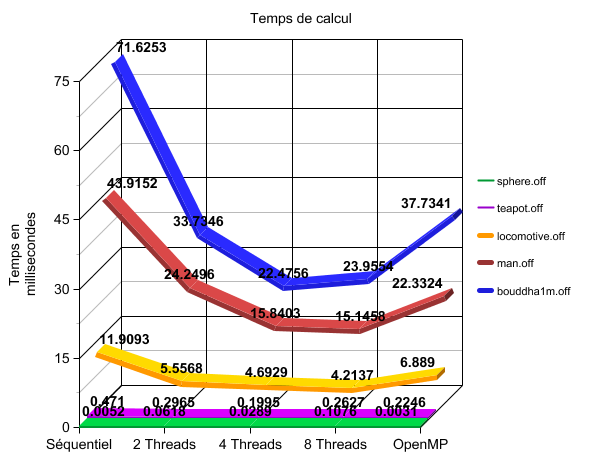
\includegraphics[scale = 0.7]{graph_execTime_machine1.png}
	\end{center}
\section{Conclusion}
% Conclusion et conjecture

\newpage
\bibliographystyle{unsrt}
\bibliography{biblio}

\end{document}
